
% ===========================
\chapter{Grundlagen}
\label{grundlagen}
% ===========================

In diesem Kapitel werden die zum Verständnis nötigen Grundlagen für diese Arbeit erklärt. Dabei wird im Abschnitt \ref{grundlagen_fahren} der Stand der Technik von automatisierten Fahrfunktionen und deren Entwicklung beschrieben. Im Abschnitt \ref{grundlagen_nn} wird maschinelles Lernen im Allgemeinen und im Speziellen künstliche neuronale Netze, die für Umsetzung dieser Arbeit nötig sind, beschrieben.


% ===========================
\section{Hochautomatisiertes Fahren}
\label{grundlagen_fahren}
% ===========================

Hochautomatisiertes Fahren wird in den vergangenen Jahren zunehmend von der Automobilindustrie vorangetrieben. Nach der Norm SAE J3016 (Abbildung \ref{fig_level_autonomes_fahren}) befinden wir uns aktuell auf Level 2 des autonomen Fahrens. Mit neuen Technologien werden immer mehr Funktionen für automatisiertes Fahren entwickelt und verknüpft. Es entstehen zunehmend komplexe Fahrfunktionen mit einer steigenden Anzahl möglicher Fahrsituationen und Szenarien \cite{king2017}. Das stellt Automobilhersteller und Automobilzulieferer vor eine große Herausforderung, da die Systemkomplexität wächst. Das schließt sowohl die Entwicklung von Assistenzsystemen als auch die dazu benötigten Testszenarien ein \cite{pfeffer2016}.

In den folgenden Abschnitten wird erläutert wie aktuell dieser Herausforderung begegnet wird. In Abschnitt \ref{grundlagen_fahren_entwicklung} wird ein allgemeiner Überblick über die aktuellen Entwicklungsmethodiken in der Automobilindustrie gegeben. Danach wird in Abschnitt \ref{grundlagen_fahren_simulation} darauf eingegangen wie die Simulation von Testfällen die aktuelle Komplexität handhabbar macht und welche Ansätze es in der Forschung dazu gibt.

\begin{figure}[h]
\centering
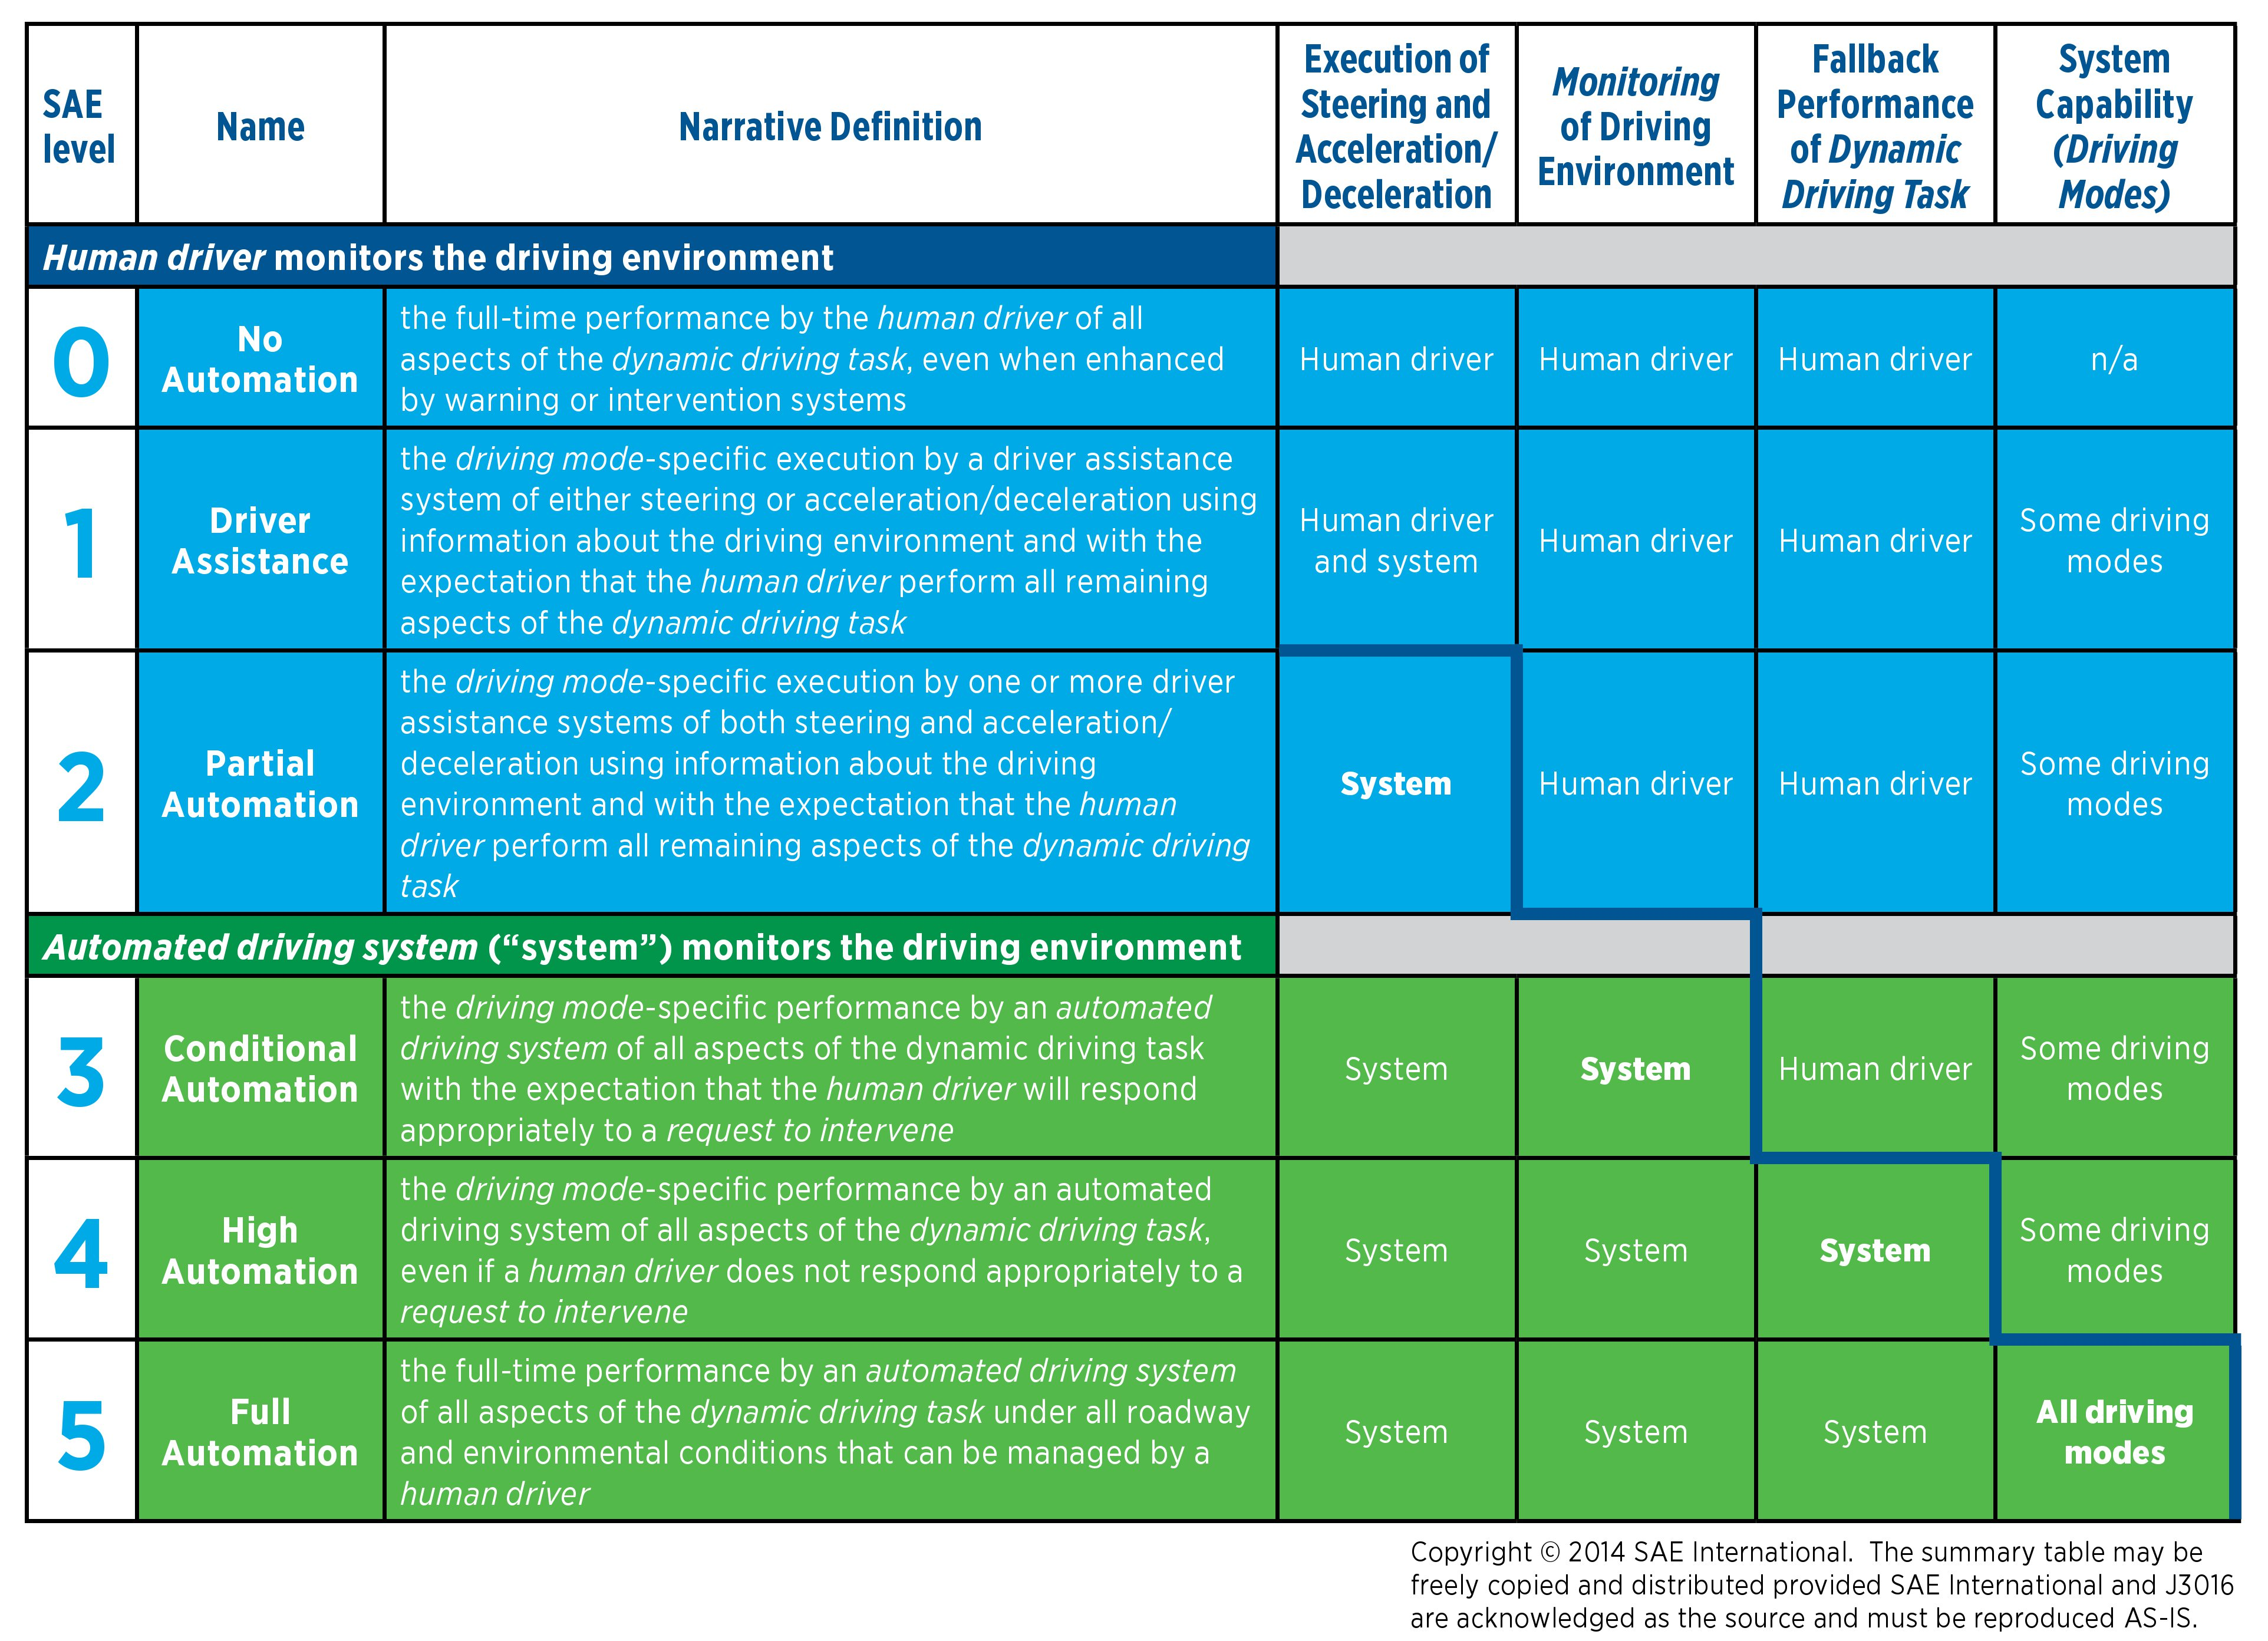
\includegraphics[scale=0.7]{level_autonomes_fahren.jpg}
\caption{Norm SAE J3016 für die Level des autonomen Fahrens, \cite{sae2014taxonomy}}
\label{fig_level_autonomes_fahren}
\end{figure}


% ===========================
\subsection{Entwicklung hochautomatisierter Fahrfunktionen}
\label{grundlagen_fahren_entwicklung}
% ===========================

HIL VIL

Lorem ipsum dolor sit amet, consetetur sadipscing elitr, sed diam nonumy eirmod tempor invidunt ut labore et dolore magna aliquyam erat, sed diam voluptua. At vero eos et accusam et justo duo dolores et ea rebum. Stet clita kasd gubergren, no sea takimata sanctus est Lorem ipsum dolor sit amet. Lorem ipsum dolor sit amet, consetetur sadipscing elitr, sed diam nonumy eirmod tempor invidunt ut labore et dolore magna aliquyam erat, sed diam voluptua. At vero eos et accusam et justo duo dolores et ea rebum. Stet clita kasd gubergren, no sea takimata sanctus est Lorem ipsum dolor sit amet. Lorem ipsum dolor sit amet, consetetur sadipscing elitr, sed diam nonumy eirmod tempor invidunt ut labore et dolore magna aliquyam erat, sed diam voluptua. At vero eos et accusam et justo duo dolores et ea rebum. Stet clita kasd gubergren, no sea takimata sanctus est Lorem ipsum dolor sit amet.

Lorem ipsum dolor sit amet, consetetur sadipscing elitr, sed diam nonumy eirmod tempor invidunt ut labore et dolore magna aliquyam erat, sed diam voluptua. At vero eos et accusam et justo duo dolores et ea rebum. Stet clita kasd gubergren, no sea takimata sanctus est Lorem ipsum dolor sit amet. 


% ===========================
\subsection{Simulation in der Entwicklung}
\label{grundlagen_fahren_simulation}
% ===========================

Lorem ipsum dolor sit amet, consetetur sadipscing elitr, sed diam nonumy eirmod tempor invidunt ut labore et dolore magna aliquyam erat, sed diam voluptua. At vero eos et accusam et justo duo dolores et ea rebum. Stet clita kasd gubergren, no sea takimata sanctus est Lorem ipsum dolor sit wie in Graph \ref{fig:x cubed graph} beschrieben.Lorem ipsum dolor sit amet, consetetur sadipscing elitr, sed diam nonumy eirmod tempor invidunt ut labore et dolore magna aliquyam erat, sed diam voluptua. At vero eos et accusam et justo duo dolores et ea rebum. Stet clita kasd gubergren, no sea takimata sanctus est Lorem ipsum dolor sit wie in Graph \ref{fig:x cubed graph} beschrieben.

Lorem ipsum dolor sit amet, consetetur sadipscing elitr, sed diam nonumy eirmod tempor invidunt ut labore et dolore magna aliquyam erat, sed diam voluptua. At vero eos et accusam et justo duo dolores et ea rebum. Stet clita kasd gubergren, no sea takimata sanctus est Lorem ipsum dolor sit wie in Graph \ref{fig:x cubed graph} beschrieben.

Duis autem vel eum iriure dolor in hendrerit in vulputate velit esse molestie consequat, vel illum dolore eu feugiat nulla facilisis at vero eros et accumsan et iusto odio dignissim qui blandit praesent luptatum zzril delenit augue duis dolore te feugait nulla facilisi.   


% ===========================
\section{Neuronale Netze}
\label{grundlagen_nn}
% ===========================

Duis autem vel eum iriure dolor in hendrerit in vulputate velit esse molestie consequat, vel illum dolore eu feugiat nulla facilisis.


% ===========================
\subsection{Maschinelles Lernen}
\label{grundlagen_nn_ml}
% ===========================

Duis autem vel eum iriure dolor in hendrerit in vulputate velit esse molestie consequat, vel illum dolore eu feugiat nulla facilisis at vero eros et accumsan et iusto odio dignissim qui blandit praesent luptatum zzril delenit augue duis dolore te feugait nulla facilisi. 


% ===========================
\subsection{Convolutional Neural Network}
\label{grundlagen_nn_cnn}
% ===========================


\begin{table}[h]
\centering
\begin{tabular}{l | l | l}
A & B & C \\
\hline
1 & 2 & 3 \\
4 & 5 & 6
\end{tabular}
\caption{very basic table}
\label{tab:abc}
\end{table}


% ===========================
\subsection{Recurrent Neural Network}
\label{grundlagen_nn_rnn}
% ===========================

Lorem ipsum dolor sit amet, consectetuer adipiscing elit, sed diam nonummy nibh euismod tincidunt ut laoreet dolore magna aliquam erat volutpat \cite{latexcompanion}. 

